\chapter*{Závěr}
\phantomsection
\addcontentsline{toc}{chapter}{Závěr}
V diplomové práci bylo navrženo a realizováno škálovatelné řešení pro měření
odporu propojení velkého množství elektrických cest. Výsledkem návrhu
je koncepce měřících a ovládacích karet, které dohromady tvoří pole 4000 pinů
mezi kterými lze libovolně měřit odpor elektrických cest. Pro obě karty
lze v příloze diplomové práce nalézt schéma zapojení a výrobní data.\par

Pro ovládací kartu byl vyvinut firmware, který ve spolupráci s PC aplikací umožňuje provádět automatická měření a
následně výsledky prezentovat ve srozumitelné grafické podobě. Dále vyvinutá PC aplikace umožňuje pohodlně
pomocí grafického rozhraní manuálně ovládat vstupy a výstupy ovládacích a měřících karet.
Dále aplikace umožňuje formátovat vstupní data,
která jsou generována nejrozšířenějšími ICT testery AGILENT (KEYSIGHT) 30xx.\par

Pro automatický běh testeru jsou k dispozici dva pracovní režimy (PASS/FAIL a měření přesného odporu).
V režimu PASS/FAIL lze proměřit propojení všech 4000 bRC
vůči jednomu vybranému bRC pinu do 40\,ms (včetně signalizace v PC aplikaci),
což splňuje požadavek na rychlost měření.\par

Funkčnost celého systému byla ověřena automatizovaným přibližně 9hodinovým měřením 
v režimu přesného měření odporu. Při tomto měření byla dosažena požadovaná přesnost,
která je definována absolutní chybou $\pm3\,\Omega$ pro rozsah $0\,\Omega$ až $100\,\Omega$ a relativní chybou
$\pm5\,\%$ pro rozsah $100\,\Omega$ až $1000\,\Omega$.\par

Výše zmíněné vlastnosti systému splňují základní požadavky na funkčnost elektrické části zařízení.
Nicméně zařízení v době odevzdání diplomové práce má několik nedostatků, které budou postupně odstraňovány
i po odevzdání práce. Prvním nedostatkem je, že ovládací karty neobsahují bootloader,
který by umožňoval aktualizaci firmwaru pomocí Ethernetu. Dále protože zatím bylo osazeno pouze 10 kusů ovládacích karet,
nebylo možné zařízení otestovat v plném rozsahu.\par

V současné době umožňuje PC aplikace načítat pouze generovaná data z ICT testerů AGILENT (KEYSIGHT) 30xx.
Do budoucna je plánováno rozšíření o další formáty dat, které jsou generovány jinými ICT testery.\par

Úkolem diplomové práce bylo realizovat mechanickou část testeru. Tato čás však není v době odevzdání dokončena.
Ve spolupráci s konstruktéry firmy Čevor Innovation a.s. byl navržen 3D model (Obrázek na další straně).
V modelu je celá logika testeru zabudovaná do stolu tvořeného hliníkovými profily.
Do stolu bude zabudováno také napájení celého zařízení, bezpečnostní prvky
v podobě start/stop tlačítka a optické závory, pneumatické části a další.
Konstrukce zařízení musí být dostatečně robustní, aby byla schopná úspěšně odolávat silám (9000\,N)
potřebným k nakontaktování všech 4000 pinů.
\clearpage

\begin{figure}[ht!]
    \centering
    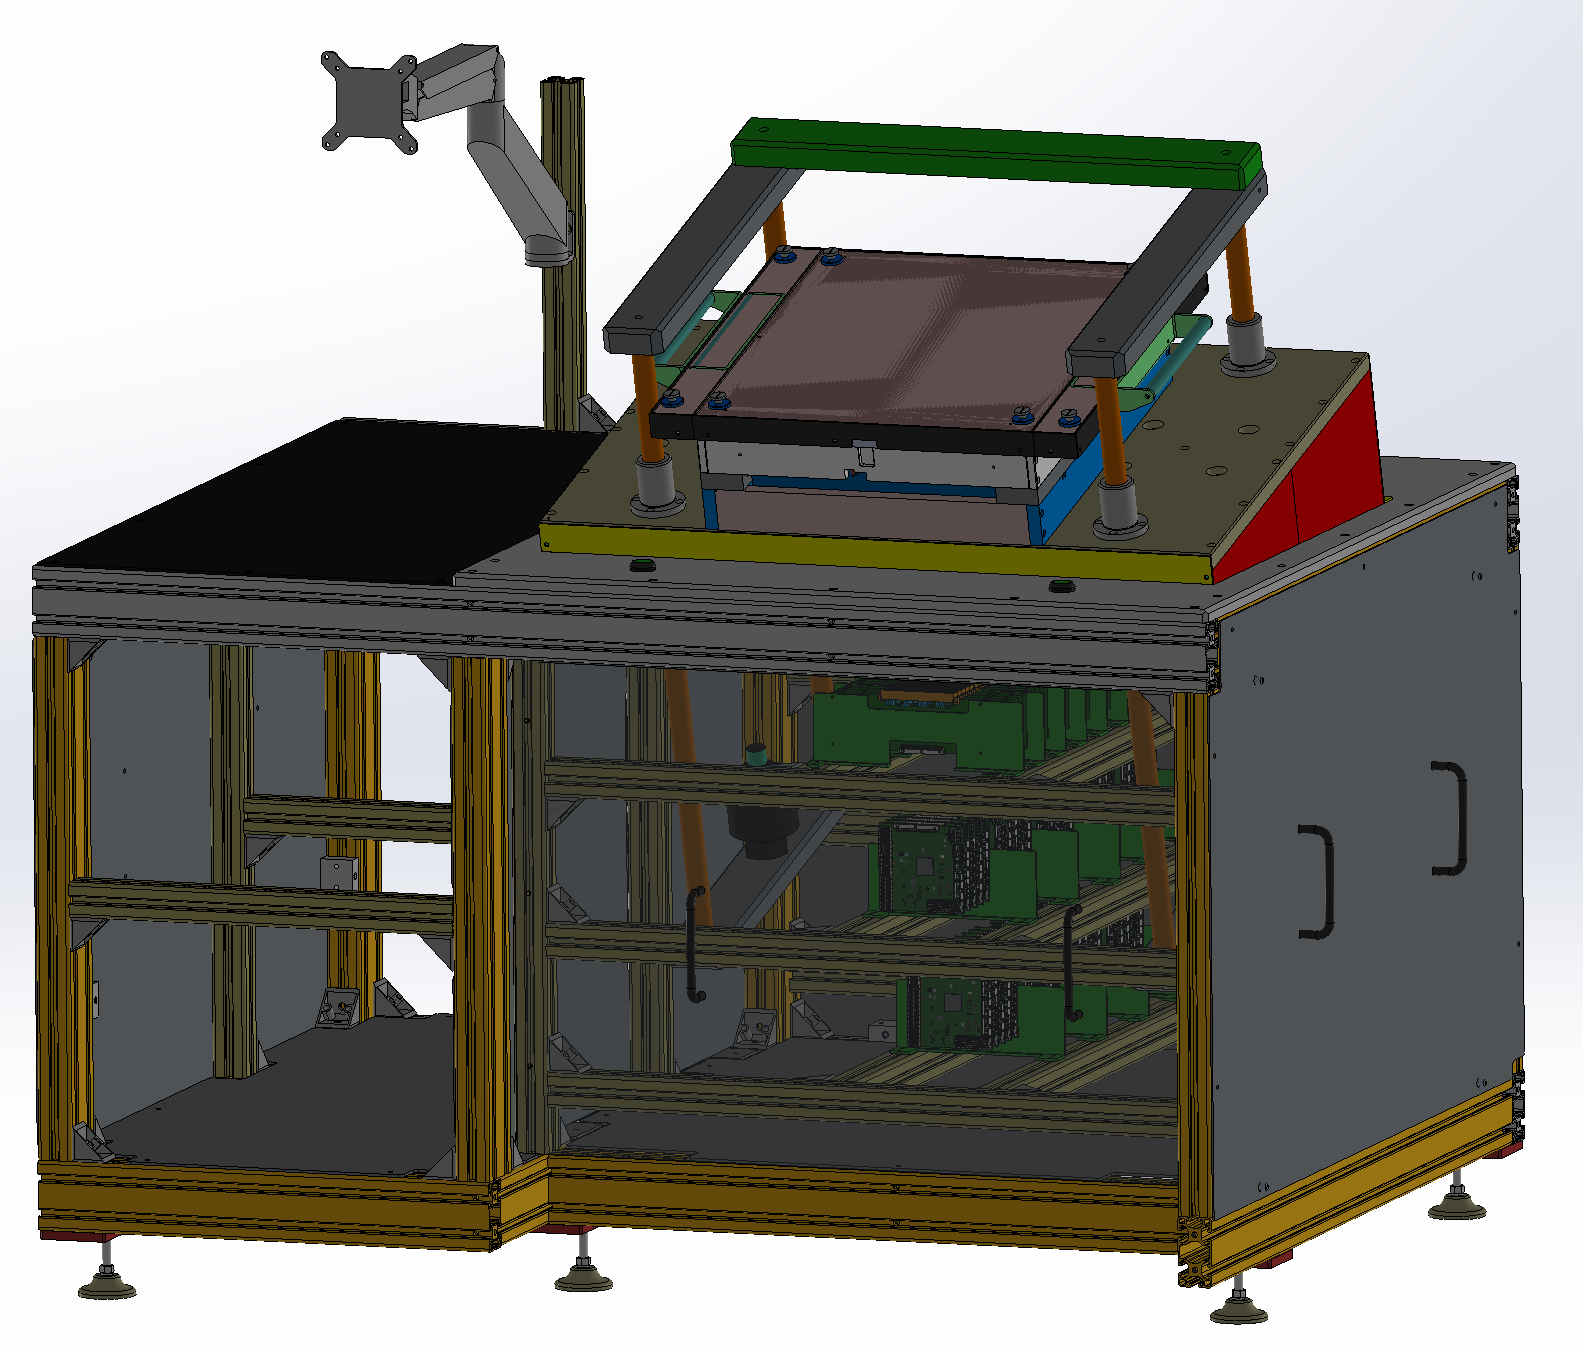
\includegraphics[width = 1\textwidth]{obrazky/assembly_3D_model.png}
    \caption{3D model mechanické části testeru}
    \label{fig: assembly model}
\end{figure}

